\section*{Problem 2 - Path Following with Crab angle Compensation}
\subsection*{Problem 2.1}
We implement a LOS guidance system using lookahead-based steering. The principle of this method is to move from one waypoint to the next by finding the LOS vector, and setting the desired course to move the vessel along this vector. Using the lookahead-based steering method, we separate the desired course a sum of the path-tangential angle and the velocity-path relative angle. The path-tangential angle can easily be found as the angle between the two waypoints, while the velocity-path relative angle can be found as using arctan of minus the cross-track error, divided by the distance between where the cross-track error and the LOS vector intercepts the line between the waypoints. 

We ended up choosing the same radius for all waypoints, set to be slightly larger than double the length of the vessel. Furthermore, we also limited delta to be between 0 and R. 

\subsection{Problem 2.2}
% \begin{figure}[ht]
% 	\centering
% 	\begin{subfigure}[b]{0.3\textwidth}
% 		\includegraphics[width=\textwidth]{}
% 		\caption{Heading}
% 		\label{fig:heading1_4}
% 	\end{subfigure}%
% 	~
% 	\begin{subfigure}[b]{0.3\textwidth}
% 		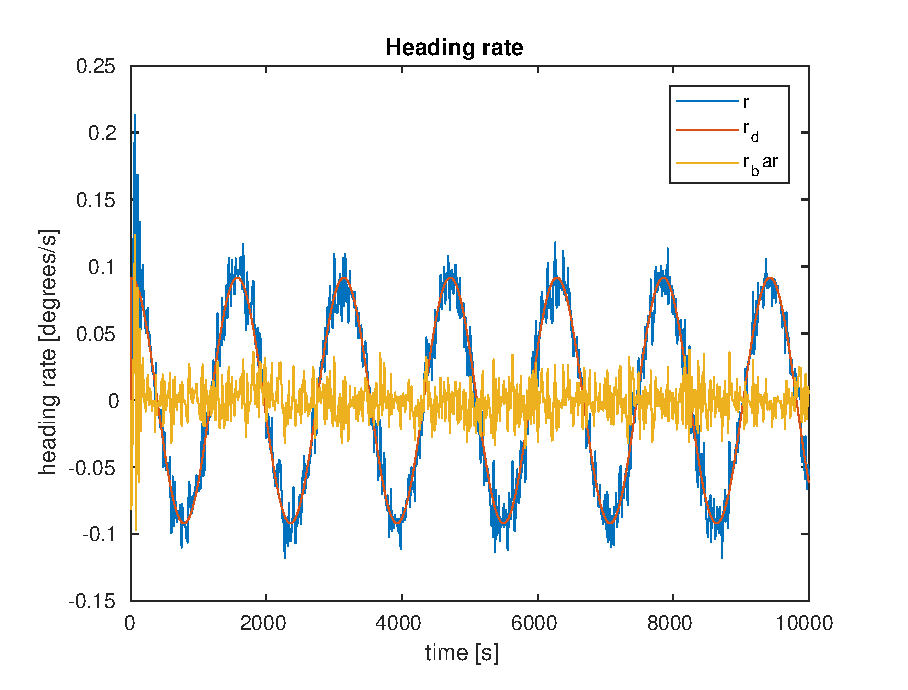
\includegraphics[width=\textwidth]{heading_rate1_4}
% 		\caption{Heading rate}
% 		\label{fig:heading_rate1_4}
% 	\end{subfigure}%
%         ~
% 	\begin{subfigure}[b]{0.3\textwidth}
% 		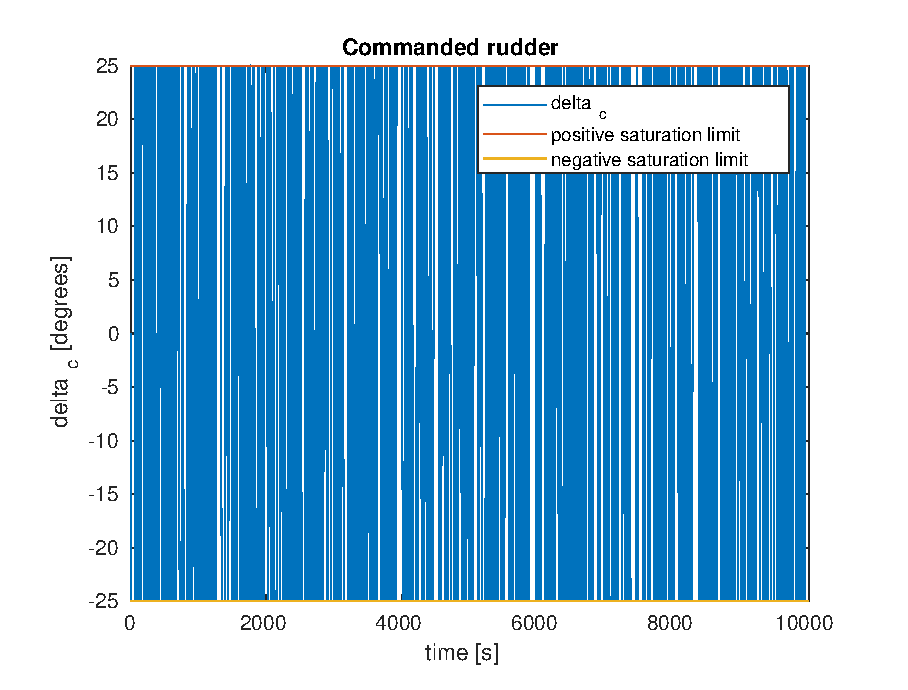
\includegraphics[width=\textwidth]{rudder1_4}
% 		\caption{Rudder with saturation}
% 		\label{fig:rudder1_4}
% 	\end{subfigure}
% 	\caption{Heading controller results}\label{fig:2}
% \end{figure}



Answer problem 2.1 here. The Greek letters for sideslip, heading and course are $\beta$, $\psi$ and $\chi$, respectively. Equation (10) in the assignment is:
\begin{equation}
\label{y_kinematics}
	\begin{aligned}
		\dot{x} &= u \cos (\psi) -v \sin (\psi) \\
		\dot{y} &= u \sin (\psi) + v \cos (\psi)
	\end{aligned}
\end{equation} 
You can refer to equations in the report by using the label and the "eqref" command. Example: equation \eqref{y_kinematics} shows the north and east velocities. 

\subsection*{Problem 2.2}
Answer Problem 2.2 here...

\subsection*{Problem 2.3}
Transfer functions can be written as
\begin{equation}
	H(s) = \frac{a_n s^n + ... + a_1 s + a_0}{b_m s^m + ... + b_1 s + b_0}
\end{equation}

The Nomoto model can be written as
\begin{equation}
\label{eq:nomoto}
	\begin{aligned}
		T \dot{r} + r &= K \delta + b \\
		\dot{\psi} &= r
	\end{aligned}
\end{equation}

\subsection*{Problem 2.4}
Answer Problem 2.4 here.  References can be placed in the "bibliography.bib" and referred to as \cite{Fossen2011} and \cite{Fjellstad1994857}. The PID-controller is
\begin{equation}
	\delta = -k_p y - k_d \dot{y} - k_i \int y
\end{equation}
